% Vector figure definitions. Both are drawn directly by TikZ/PGFPlots.
\pgfplotsset{
  paperplot/.style={
    tick label style={font=\scriptsize},
    label style={font=\scriptsize},
    grid style={black!10},
    axis line style={black!75},
    tick style={black!75},
    clip=false,
  }
}

\newcommand{\SixModelEffectsPlot}{%
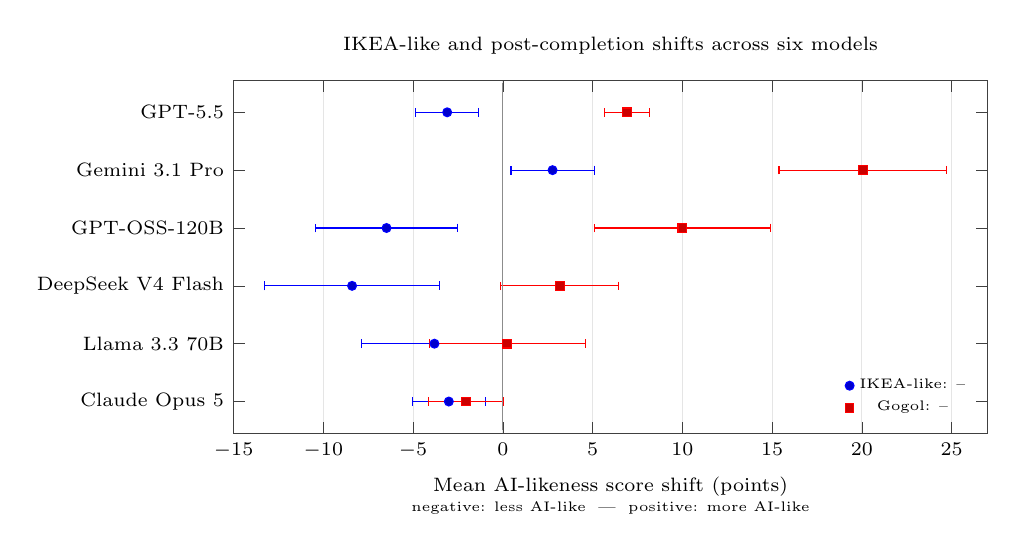
\begin{tikzpicture}[font=\scriptsize]
\begin{axis}[
  width=.92\linewidth,
  height=.50\linewidth,
  xmin=-15, xmax=27,
  xtick={-15,-10,-5,0,5,10,15,20,25},
  ymin=-0.55, ymax=5.55,
  y dir=reverse,
  ytick={0,1,2,3,4,5},
  yticklabels={GPT-5.5,Gemini 3.1 Pro,GPT-OSS-120B,DeepSeek V4 Flash,Llama 3.3 70B,Claude Opus 5},
  paperplot,
  title style={font=\scriptsize},
  title={IKEA-like and post-completion shifts across six models},
  xlabel={\shortstack{Mean AI-likeness score shift (points)\\[-1pt]\tiny negative: less AI-like \;|\; positive: more AI-like}},
  xmajorgrids,
  legend style={
    at={(0.99,0.02)}, anchor=south east,
    draw=none, fill=none,
    font=\tiny,
    row sep=-1pt,
  },
]
\addplot+[
  only marks, mark=*, mark size=1.6pt,
  error bars/.cd, x dir=both, x explicit,
] table[x=x,y=y,x error minus=em,x error plus=ep,row sep=\\]{
 x      y   em      ep\\
-3.10   0   1.766   1.763\\
 2.77   1   2.316   2.319\\
-6.48   2   3.967   3.974\\
-8.40   3   4.861   4.861\\
-3.81   4   4.077   4.075\\
-3.01   5   2.031   2.027\\
};
\addlegendentry{IKEA-like: \replay{}--\live{}}
\addplot+[
  only marks, mark=square*, mark size=1.55pt,
  error bars/.cd, x dir=both, x explicit,
] table[x=x,y=y,x error minus=em,x error plus=ep,row sep=\\]{
 x      y   em      ep\\
 6.91   0   1.267   1.272\\
20.06   1   4.673   4.663\\
10.00   2   4.905   4.900\\
 3.18   3   3.288   3.278\\
 0.24   4   4.343   4.342\\
-2.05   5   2.100   2.106\\
};
\addlegendentry{Gogol: \post{}--\replay{}}
\draw[black!45,thin] (axis cs:0,-.5) -- (axis cs:0,5.5);
\end{axis}
\end{tikzpicture}
}

\newcommand{\ReliabilityMapPlot}{%
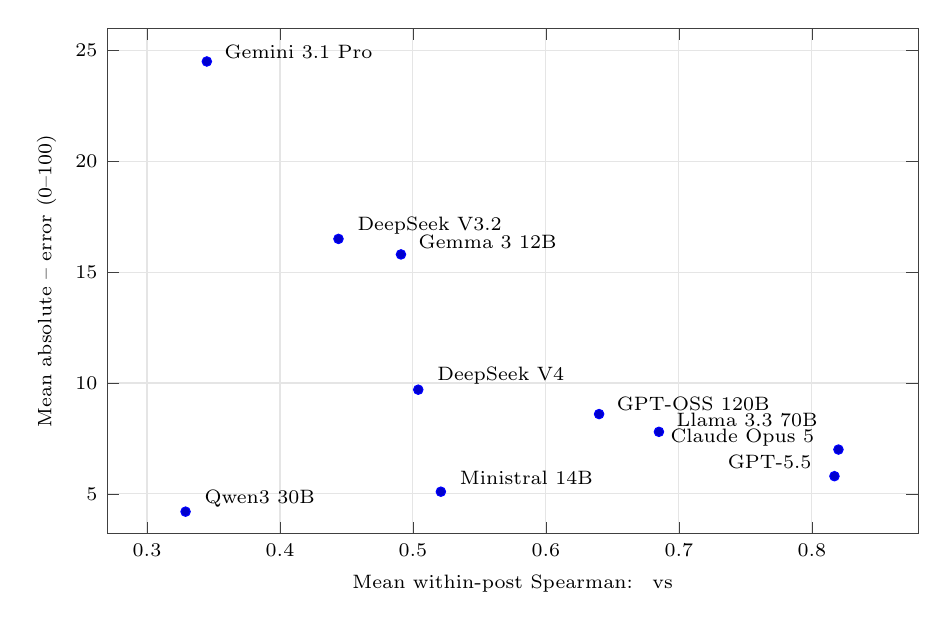
\begin{tikzpicture}[font=\scriptsize]
\begin{axis}[
  width=.98\linewidth,
  height=.66\linewidth,
  xmin=.27, xmax=.88,
  ymin=3.2, ymax=26.0,
  xtick={.3,.4,.5,.6,.7,.8},
  ytick={5,10,15,20,25},
  xlabel={Mean within-post Spearman: \live{} vs \post{}},
  ylabel={Mean absolute \live{}--\post{} error (0--100)},
  paperplot,
  xmajorgrids, ymajorgrids,
]
\addplot+[only marks, mark=*, mark size=1.7pt] coordinates {
  (.820,7.0) (.817,5.8) (.685,7.8) (.640,8.6) (.521,5.1)
  (.504,9.7) (.491,15.8) (.444,16.5) (.345,24.5) (.329,4.2)
};
\node[anchor=west] at (axis cs:.351,24.95) {Gemini 3.1 Pro};
\node[anchor=west] at (axis cs:.451,17.10) {DeepSeek V3.2};
\node[anchor=west] at (axis cs:.497,16.38) {Gemma 3 12B};
\node[anchor=west] at (axis cs:.511,10.35) {DeepSeek V4};
\node[anchor=west] at (axis cs:.646,9.05) {GPT-OSS 120B};
\node[anchor=west] at (axis cs:.691,8.35) {Llama 3.3 70B};
\node[anchor=east] at (axis cs:.809,7.55) {Claude Opus 5};
\node[anchor=east] at (axis cs:.807,6.45) {GPT-5.5};
\node[anchor=west] at (axis cs:.528,5.75) {Ministral 14B};
\node[anchor=west] at (axis cs:.336,4.80) {Qwen3 30B};
\end{axis}
\end{tikzpicture}
}
